% Sidebar subcategory icon: Element order & topology — one triangle carrying
% both its corner nodes and its mid-edge nodes, i.e. element ORDER as such.
% Distinct from `quadratic` (a linear→quadratic pair joined by an arrow), which
% is the icon of a single operation inside this category.
% Drawn coarser than an operation icon on purpose: a .sb-subsection-header
% renders it at 14px, so anything under ~2 units of this 24-unit grid vanishes.
% NOTE: the committed svg-ui/catTopology.svg was hand-authored to the same
% drawing (no pdftocairo available); regenerating via `make ui` replaces it with
% the pdftocairo rendering of this source — same glyph either way.
\documentclass[tikz,border=2mm]{standalone}
\usetikzlibrary{arrows.meta,calc,shapes.geometric}
\begin{document}
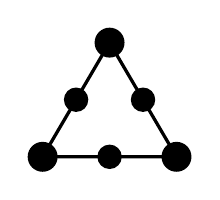
\begin{tikzpicture}[line width=1.3pt, line cap=round, line join=round, x=1mm,y=1mm]
  \coordinate (A) at (-8.5,-7);
  \coordinate (B) at (8.5,-7);
  \coordinate (C) at (0,7.5);
  \draw[line width=1.18pt] (A) -- (B) -- (C) -- cycle;
  \fill (A) circle (1.9);
  \fill (B) circle (1.9);
  \fill (C) circle (1.9);
  \fill ($(A)!0.5!(B)$) circle (1.55);   % mid-edge nodes
  \fill ($(B)!0.5!(C)$) circle (1.55);
  \fill ($(C)!0.5!(A)$) circle (1.55);
\end{tikzpicture}
\end{document}
